\setchapterpreamble[o]{%
\dictum[--- \textsc{Louis Pasteur}]{\Gun Theorie ist die Mutter der Praxis.\Gob}}
\renewcommand{\chapterheadstartvskip}{\vspace*{2cm}}

\chapter{Theoretische Grundlagen}
\label{chap:theoretischegrundlagen}

In diesem Kapitel werden die theoretischen Grundlagen erläutert die benötigt werden, um die Forschungsfrage zu beantworten.
Zunächst MPC dann eher technisch

\section{Model Predictive Control}
\label{chap:mpc}


\acrlong{mpc} an sich ist eine Methodik zur Steuerung von Systemen. Diese versucht zunächst, zu sich periodisch wiederholenden, diskreten Zeitpunkten das Verhalten eines Systems in der Zukunft -- also einer immer gleich weit in die Zukunft hineinreichenden Periode -- zu beschreiben. Hierzu bedient \acrlong{mpc} sich der Kenntnis des aktuellen Zustandes und eines physikalischen-mathematischen Modells des Systems, um dessen zukünftiges Verhalten \Gun vorherzusagen \Gob bzw. abzubilden. Des Weiteren wird versucht das Verhalten des Systems mit minimalem Aufwand zu beeinflussen, um einem eigens- oder vordefinierten Zielkriterium zu folgen \acrlong{bzw} diesem zu entsprechen.




\section{Technische Grundlagen zur Kommunikation mit Bussystemen}
\label{sec:grundlagenbus}
In diesem Kapitel werden die Grundlagen von Hard- und Software beleuchtet die für die Kommunikation der Steuerung mit den einzelnen Anlagenteilen benötigt werden.
Diese umfassen zunächst Bussysteme im Allgemeinen und werden anhand des spezifischen/konkreten Anwendungsfalls Modbus erläutert.
Die Einführung wird sich an die Struktur nach \cite{schn06} anlehnen.

\subsection{OSI-Kommunikationsmodell}
Aufgrund der großen Anzahl verschiedener technischer Systeme existieren auch viele verschiedene Arten der Kommunikation untereinander. Bei der genaueren Betrachtung der Kommunikation wird ersichtlich, dass diese oftmals ähnlich abläuft und sich durch ein Meta-Schema beschreiben lässt \cite[S.~8]{schn06}. Um die Kommunikation auch über verschiedenen Systeme hinweg zu ermöglichen und sie zu formalisieren, wurde von der \textit{International Organization for Standardization} 1984 ein abstraktes Referenz-Modell entwickelt, dass in der \textit{ISO-Norm 7498-1} beschrieben ist. Es dient der Entwicklung und Verbesserung von Standards für den Informationsaustausch sowie als Referenz für bestehende Standard um eine gewisse Konsistenz zu wahren \cite[S.~1]{osi96}. Das Ziel bei dem Entwurf des Modells war es, eine Menge von Standards zu schaffen um autonomen Systemen die Kommunikation untereinander zu ermöglichen \cite[S.~4]{osi96}.

Das sogenannte \acrlong{osi} wird zunächst allgemein erläutert, da die Kommunikation von technischen Systemen im Rahmen der Arbeit eine zentrale Rolle spielt, und wird anschließend im Anwendungskontext mit den eingesetzten Protokollen und Schnittstellen referenziert.

Zunächst wird im Standard definiert, womit sich das Modell beschäftigt und abgegrenzt welche Aspekte im Modell keine Berücksichtigung finden \cite[S.~3]{osi96}:

\begin{quote}
\textit{\Gun OSI is concerned with the exchange of information between open systems (and not the internal functioning of each individual real open system).\Gob}
\end{quote}

Das \acrshort{osi} beschäftigt sich also zentral mit dem Austausch von Informationen zwischen verschiedenen offenen Systemen und allen dabei anfallenden Aktivitäten. Diese sind sehr umfangreich und lassen sich in folgende Bereiche gliedern \cite[S.~3f.]{osi96}:

\begin{itemize}
	\item Der Austausch von Informationen zwischen offenen Systemen,
	\item die physischen Medien zur Verbindung von offenen Systemen und deren Transportmöglichkeit von Informationen,
	\item die Vernetzung von offenen Systemen,
	\item die Interaktion zwischen offenen Systemen und deren Fähigkeit zur Kooperation bei der Datenübertragung.
\end{itemize}

Bezogen auf den Austausch von Informationen überschneiden sich die physische Verbindung und die Vernetzung und entsprechen zusammen der Infrastruktur und deren Architektur, die zur Übertragung zur Verfügung steht. Die Interaktion umfasst weitaus mehr Aufgaben: Neben der Synchronisation der Prozesse, die Daten austauschen wollen, muss auch die Darstellung der auszutauschenden Daten und eventuell notwendige Transformationen beachtet werden, um eine Kompatibilität unterschiedlicher Systeme zu erreichen. Weitere wichtige Aufgaben sind die Datenspeicherung, deren Integrität und die Sicherheit beim Austausch hinsichtlich Fehler und Einsicht von Außen \cite[S.~4]{osi96}.
Es ist leicht zu erkennen, dass die technische Kommunikation einen sehr umfangreichen und komplizierten Prozess darstellt. Daher wird der Kommunikationsprozess im \acrshort{osi} stark abstrahiert und in sieben abstrakte Ebenen gegliedert. Die einzelnen Ebenen sind in \ref{fig:osi} dargestellt und dienen dazu verschiedene Aufgaben des Kommunikationsprozesses in Teilaufgaben zusammenzufassen.

\begin{figure}
\centering
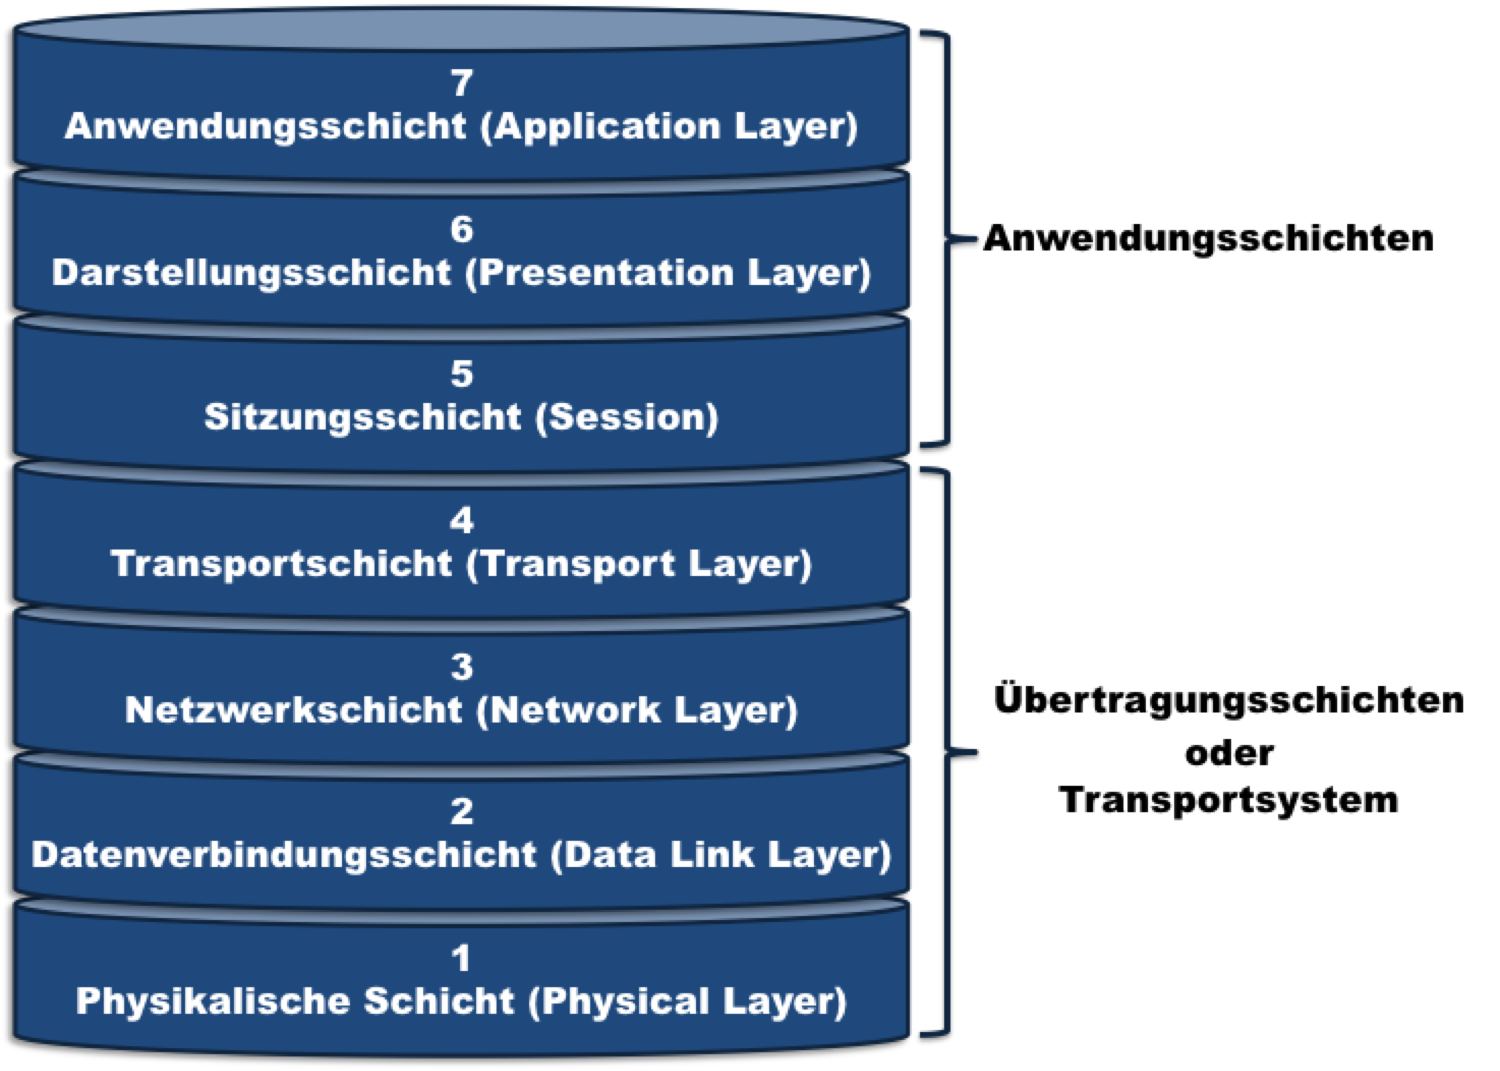
\includegraphics[width=\textwidth]{abbildungen/20160112_osi}
\caption[Die sieben Schichten des Open System Interconnection Modells]{Die sieben Schichten des \textit{Open System Interconnection} Modells verändert nach \cite[S.~10]{schn06} und \cite[S.~28]{osi96}}
\label{fig:osi}
\end{figure}

Die Ebenen werden Schichten genannt und haben klar definierte Aufgaben und Schnittstellen zu ihren Nachbarschichten. An diesen Schnittstellen werden Dienste bereitgestellt, die von den anderen Ebenen genutzt werden können. Durch diesen Aufbau können einzelne Schichten einfach bearbeitet oder ausgetauscht werden, ohne die Gesamtfunktionalität zu gefährden. Außerdem kann ein System auch aus Komponenten verschiedener Hersteller zusammengesetzt werden, womit diese Architektur nachweislich als Basis für offene Systeme dient. In \ref{fig:osi} ist ebenfalls dargestellt, dass die Schichten eins bis vier auch als Übertragungsschichten beziehungsweise Transportsystem zusammengefasst werden, weil sie für die Datenübertragung zwischen Systemen als gemeinsame Aufgabe haben. Die Schichten fünf bis sieben werden als Anwendungsschichten bezeichnet weil sie bei der Datenübertragung die Zusammenarbeit zwischen der Anwendersoftware und dem Betriebssystem sicherstellen \cite[S.~8f.]{schn06}.

Die Schnittstellen/Dienste zwischen den Schichten werden als Service Access Points bezeichnet und besitzen jeweils eine eindeutige Adresse, die oberhalb liegende Schicht ist der Service user, da er den Service daer unterhalb liegenden Schicht nutzt, dem service provider. Die Dienste können in verbindungsorientierte und verbindungsunabhängige unterschieden werden. 
Bei der Abhandlung der Dienstaufgaben stehen vier Dienstvorgänge zur Verfügung, die zusammengefasst in \ref{fig:vorgang} abgebildet sind:
request - Anforderung
indication - Meldung
response - Antwort
confirmation - Bestätigung
Bestätigten Diensten stehen alle vier Vorgänge zur Verfügung, unbestätigten lediglich die Anforderung und Meldung.
Typische Dienste sind Connect, disconnect, data

\begin{figure}
\centering
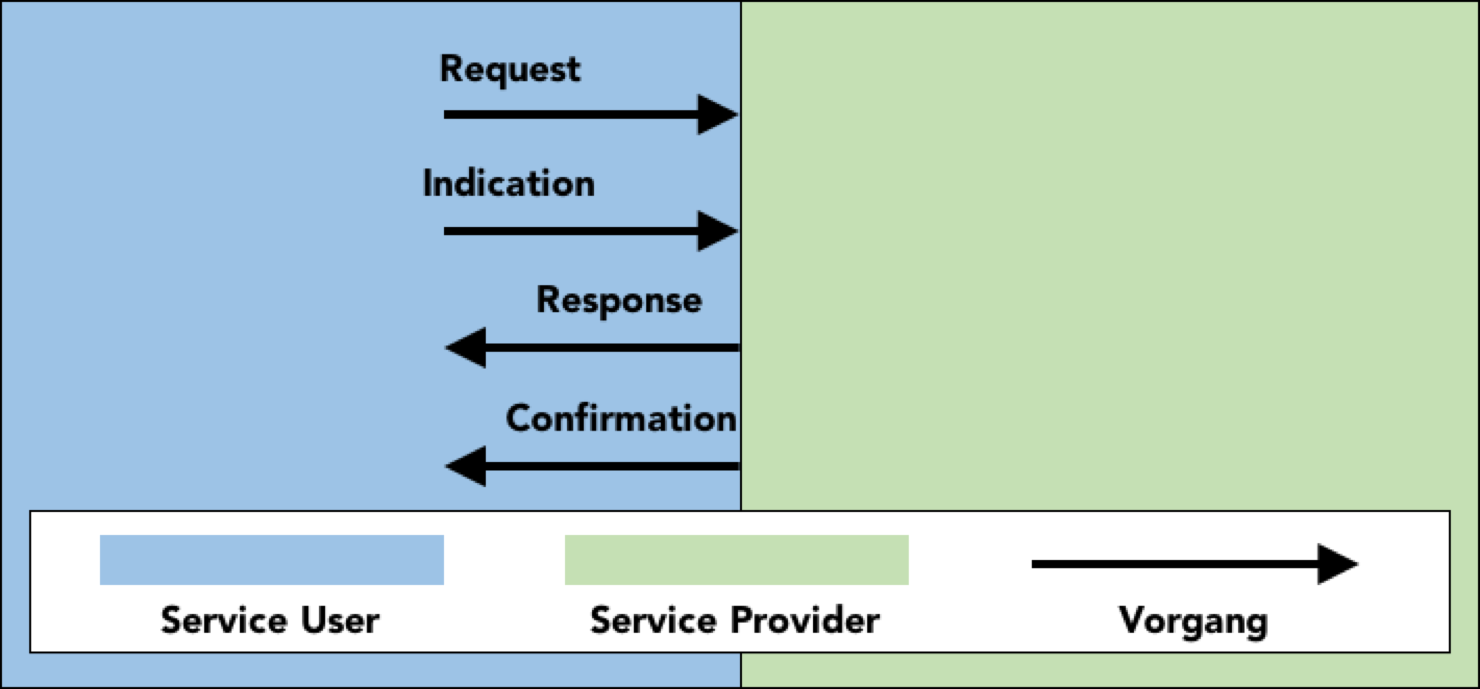
\includegraphics[width=\textwidth]{abbildungen/20160310_vorgang}
\caption{Die vier Dienstvorgänge}
\label{fig:vorgang}
\end{figure}

\cite[S.~14f.]{schn06}.

Im Folgenden wird kurz auf die einzelnen Schichten von Unten nach oben eingegangen bevor das Zusammenwirken der einzelnen Schichten anhand eines Beispiels verdeutlicht wird. %Evtl raus

Die erste, physikalische Schicht stellt die mechanischen und elektrischen Möglichkeiten zur physischen Verbindung von Systemen zur Verfügung, um die Datenübertragung der einzelnen Bits zu ermöglichen \cite[S.~49f.]{osi96}. Sie legt also die mechanischen und elektrischen Eigenschaften der Übertragung fest, also die Endsystemkopplung (Stecker), die Kabelspezifikationen und die Zuordnung der Anschlüsse sowie die Art der Codierung und die Spannungspegel zur Übertragung. In der Regel werden dazu bestehende Normen genutzt, wie zum Beispiel die elektrischen Übertragungsstrecke nach RS485-Norm, welche im Folgenden noch erläutert wird.

Ein wichtiger Aspekt der Schicht ist es, dass die Spezifikation der Strecke und nicht das physikalisches Medium selbst Teil der Schicht eins ist, denn die Kommunikation ist unabhängig von der konkreten Ausprägung der Schicht \cite[S.~9]{schn06}.

%Here We Go
Die zweite Schicht betrachtet Kommunikation zwischen zwei systemen. Deshalb stellt die Datenverbindungsschicht, stellt funktionale und prozedurale Möglihckeiten für den verbiindungsaufbau/trennung erhaltung und den Transfer von Dateneinheiten Verfügung. Ermögliocht dem Netzwerkschucht die Kontrolle über die Verbindung von Data circuits physikalisch, sowie fehlerabfangen der physikalsichen schicht \cite[S.~46f.]{osi96}
Aufgabe ist sicherer transport von Station zu station. Datensicherung --> Verpacken um Übertragungsfehler erkenntlich zu machen in data frames. In Frames sind die maximale Anzahl Datenbits für Rohdaten spezifiziert, weiterhin wird Information zur Übertragung hinzugefügt. Die zusatzinfo kann Prüfsumme und Anfang und Ende des Rahmens enthalten oder quittierung eines telegramms und dient dazu fehlerhafte Übertragung oder etwas verloren gegangen zu überprüfen. MAC mit Schicht eins, LLC mit Schicht drei.
Wuelle Wiki bisher
MAC regelt den Zugriff auf das ohyische Medium zur Kommunikation, kotrolliert oder konkurriert.
LLC verteilt die Daten passend in Schicht drei und gibt die Daten von schihct drei an passende MAC für schicht eins weiter und fügt Diese Infos von oben hinzu (Adressen Empfönger und Sender und zusatzinfo wie control für Steurung von Datenfluss oder so).

Wichtig Die schicht hat jedoch keine Kenntnis über Inhalte der Daten!\cite[S.~9ff.]{schn06}

% EIG bei 3 evtl schon bei 2 mit LLC in zusammenahng
verbindungsloser Dienst heisst keine Verbindung zwischen Kommunikationspartnern, Datenpakete werden wie Brief ganz in Netzwerk gespeist mit Zieladresse versehen und weitertransportiert, ohne beeinflussung des transportweges durch benutzer des netzwerkdienstes. Später ist Modbus ein Beispiel dazu erklärt.
verbindungsorientierte Dienste heisst ein virtueller Kanal zwischen kommunikationspartnern wird zur Verüfung gestellt, eingeriechtet: Verbindungsaufbau, Datenautausch, Verbindungsabbau, wie telefongespräch. \cite[S.~11f.]{schn06}


Die dritte Schicht beschäftigt sich mit dem Netzwerk als Ganzes. Die Aufgaben der Netzwerkschicht hängen ein wenig ab von verbindungsorientierung Daher beschäftigt sie sich mit dem Aufbau , der erhlatung und Datenaustasuch und dem trennen von Netzwerk Verbindungen zwischen offenen systemen i Netzwerk, also schnittstellen. weietrhin ist sie für den Transport von Daten im netzwerk zustaändig, also insbeonsdere auch für die Festelgung der Route(Wegsteuerung) der Daten im Netzwerk \cite[S.~41f.]{osi96}.
Also Kontrolle von Verkehr im Netzwerk, d.h. Anzahl Pakete im Netzwerk, Staus \cite[S.~11f.]{schn06}


Die vierte Schicht ist die Transportschicht und zuständig für die transparente Übertragung von Daten zwischen Prozessen und ist völlig unabähngig bzw losgelöst von den Gedanken an Kosten und Verlässlichkeit der Datenübertragung, da dies aufgaben der unteren schichten sind. Sie kümmert sich um die optimale nutzung von Netzwerk services/Nutzung \cite[S.~37f.]{osi96}.
Adressierung der Teilnehmer, Aufbau und Abbau für Transportverbindung wzischen Kom.Partner prozessen(Sammel Einzel Mehrere), Fehlerbehalndlung verbidnung und flusskontrolle, Synchronisierung der dtaenaustauschenden Prozesse.Zerlegung der Daten aus Sitzugnsschicht in Transportierbare Einheiten. Internetworking, Umsetzung verschiedener Protokolle Gateway Aufgaben. Aufbau Verbindung legt Art fest, Punkt zu Punkt oder Broadcast/Multicast (Alle bzw einige Teilnehmer gleichzeitig) \cite[S.~12f.]{schn06}.

Die fünfte Schicht, die Sitzungsschicht, startet eine Sitzungsverbindung mit bestimmter Adresse wenn dieser Prozess von einer höheren Schicht angefordert wird. Diese Verbindung dient dazu, den  dialog von kooperiendnen Porzesse auf der eines höhreren Darstellungsbene durch eine Sitzungsverbindung zu synchronisieren und deren Datenaustausch zu organisieren. verknüpft die Sitzungsadressen mit den Transportadressen, also die Anwendungsschiten mit dem Transportsystem \cite[S.~35]{osi96}.
Benutzung des Transportsystems über die Schnittstelle zur Transportschicht. Je nach Funktionen der höheren Schihcten entsprechender Funktionsumfang
BCS Basic Combined Subset - Verbindungssteuerung und Datenübertragung
BAS Basic Activity Subset - Aktivitätsverwaltung
BSS Basic synchronized Subset - Synchronisierung
\cite[S.~13]{schn06}.


Die sechste Schicht, die Darstellungsschicht ist nach \cite[S.~33f.]{osi96} für die Darstellung der Daten die von Anwendung-Entitäten entweder kommuniziert oder bei deren Kommunikation referenziert werden. Sie stellt außerdem eine gemeinsame Represantion der übertragenen Daten dar zwischen Anwendungs-Entitäten und befreit diese dadurch von Syntaxabhängigkeiten.
\cite[S.~13f.]{schn06} stellt fest, dass die Dienste die der Darstellung der transferierten Daten dienen wie die Codierung der zu übertragenden Daten, der verwendete Zeichensatz und die Darstellung der Daten auf dem Bildschirm oder Drucker. Semantik/Syntax beim Nachrichtenaustausch und der beiden Kommunizierenden Prozesse. Evtl Komprimierung um Zeit und Kosten zu sparen .


Die siebte und letzte Schicht stellt lediglich eine Möglichkeit für Anwendungsprzesse zur Verfügung um auf die OSI Umgebung zuzugreifen. Jeder Anwendung stellt im OSI genau einen Anwendungsprozess dar, verschiedene Anwendungsprozesse für verschiedene Anwendungen und vice versa \cite[S.~32]{osi96}
stellt Funktionen bereit, mit denen der Benutzer auf das Kommunikationssystem zugreifen kann, wobei der Benutzer idR ein Computerprogramm und kein Mensch ist. \cite[S.~14]{schn06}



\subsection{Bussysteme} 
Um ganz allgemein Prozesse überwachen und steuern zu können müssen unter den einzelnen Einheiten innerhalb eines Systems Informationen ausgetauscht werden. Dazu werden Kommunikationssysteme benötigt mit Hilfe derer Kommunikation erfolgen kann. Diesem Zweck dienen Bussysteme
Info/Quelle 
%%W. Kriesel, T. Heimbold, D. Telschow: Bustechnologien für die Automation, Hüthig GmbH, Heidelberg 1998
Bussysteme lassen sich anhand verschiedener Kriterien einteilen bzw klassifizieren. Im Rahmen dieser Arbeit wird der Modbus eingesetzt weshalb im Folgenden die Kriterien zunächst sehr allgemein zum Verständnis des Krieteriums beschrieben werden. Die verschiedenen Ausprägungen der einzelnen Kriterien werden lediglich die für Modbus relevanten detailliert beschrieben.

\subsubsection{Netzwerk und Topologie}
Verknüpft man einzelne Prozesseinheiten -- im folgenden Teilnehmer des Netzwerks -- miteinander über Verbindungsleitungen, über die Informationen übertragen werden können, entstehen dabei Netzwerke. Diese Netzwerke können unterschiedlich ausgeprägt sein und werden anhand ihrer geometrischen Anordnung, der Netzwerktopologie, unterschieden.
--> Teilnehmer im Netzwerk definieren

Die einfachste Art zwei Teilnehmer miteinander zu verbinden ist eine direkte Zweipunktverbindung mit einer Leitung. Jedoch würde mit jeder steigenden Zahl von Teinehmern auch überproportional mehr Verbindungsleitungen benötigt um alle Teilnehmer miteinander zu verbinden. Dies hätte für große Zweipunbktverbindungsnetzwerke. die auch als vermaschtes Netz bezeichnet werden, eine unübersichtliche große Anzahl von Schnittstellen, einen extrem hohen Verkabelungsaufwand und damit verbundene hohe Kosten zur Folge. Um dies zu vermeiden ergeben sich noch verschiedene andere Möglichkeiten zur Anordnung von Teilnehmern in Netzwerken \cite[S.~1f.]{schn06}.

Die Zweipunktverbindungen sind wie oben beschrieben mit einem hohen Verkabelungsaufwand verbunden, weshalb bei großen Netzwerken oftmals zu einer Linienstruktur übergegangen wird. Diese wird auch Linienstruktur genannt und wird auch von der Modbus-Technologie empfohlen/vorgeschrieben. Charakteristisch dafür ist, dass alle Teilnehmer eine gemeinsame Verbindungsleitung zur Kommunikation nutzen. Dazu gibt es ein sogenanntes, langes Buskabel entlang dessen die einzelnen Teilnehmer mit Hilfe von kurzen Stichleitungen angebunden sind, wie auf Abbildung \ref{fig:bus_struktur} zu sehen ist.

\begin{figure}
\centering
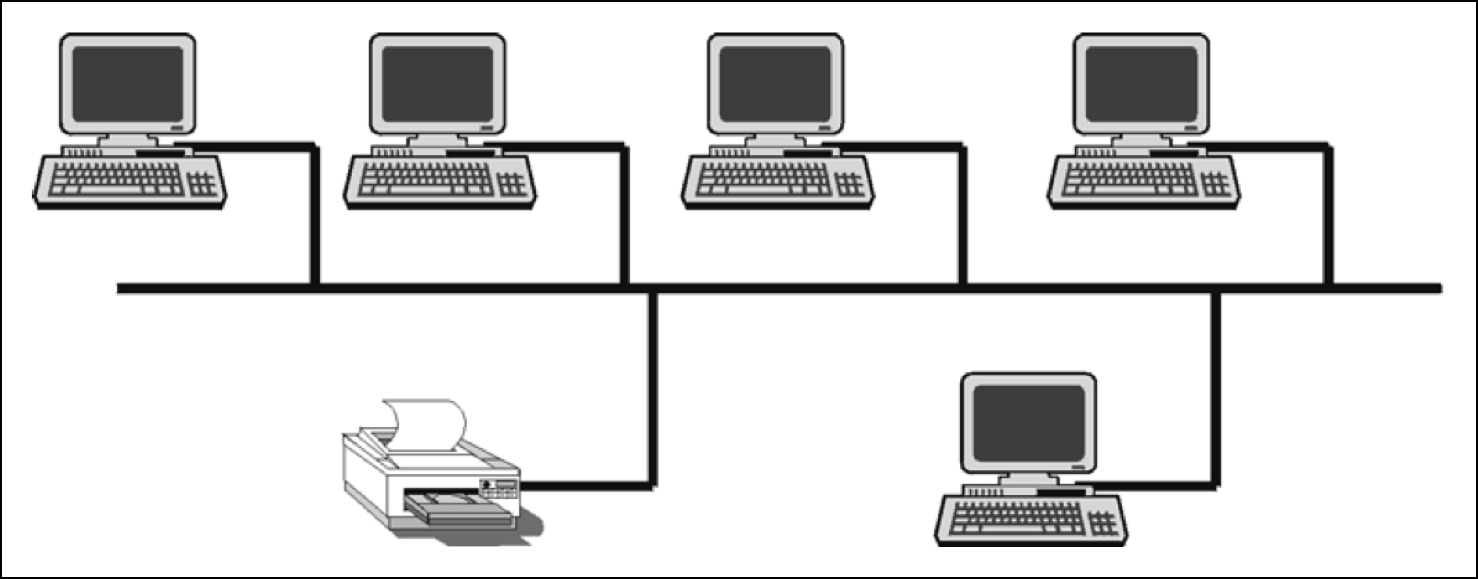
\includegraphics[width=\textwidth]{abbildungen/20160109_busstruktur}
\caption[Linienstruktur]{Linienstruktur aus \cite[S.~3]{schn06}}
\label{fig:bus_struktur}
\end{figure}

Dadurch wird der Verkabelungsaufwand auch für sehr große Netzwerke stark reduziert und auch die Anzahl an Schnittstellen der Teilnehmer auf eine einzige reduziert. Jedoch wird dadurch das gleichzeitige Senden von Teilnehmern erschwert und es müssen sogenannte Buszugriffsverfahren definiert werden, die nichts weiter als Regeln sind die den Zugriff auf den Bus festlegen. Da die Kommunikation auf einer einzigen Leitung stattfindet und ständig alle Teilnehmer alle Sendungen verfolgen wird der Sender durch diese Parallelschaltung der Empfänger stark belastet. Da die Bus-Längen meist sehr lang sind ( hunderte Meter) ist die Leitungslänge im Bezug auf die zu übertragende Wellenlänge nicht mehr vernachlässigbar. Deshalb müssen beide Enden der Busleitung mit Leitungsabschlusswiderständen versehen werden sowie die Leitungslänge und die Teilnehmer je Netzwerk begrenzt werden. Der Leistungs- und Kapazitätswiderstand einer Leitung sind von der Länge der Leitung abhängig und werden durch das Ersatzschaltbild eines RC-Gliedes repräsentiert, wie in Abbildung \ref{fig:bus_impuls}a zu sehen ist. Durch diese Widerstände wird eine Impulsverzerrung $\delta t$ auf der Leitung ausgelöst, die somit mittelbar auch von der Leitungslänge abhängt. Je länger die Leitung desto größer die beiden Widerstande und desto größer ist die Impulsverzerrung $\delta t$, da der Kondensator C\_{Leitung} mehr Zeit zum Aufladen benötigt und die Lastspannung sinkt, wie in Abbildung \ref{fig:bus_impuls}b und \ref{fig:bus_impuls}c dargestellt. Dadurch wird die maximale Frequenz der Datenübertragung beschränkt (auf den Kehrwert der Impulsverzerrung f=1/t). Dies bedeutet das die Frequenz der Datenübertragung entlang der Leitung von ihrer Länge mittelbar abhängig ist, da ansonsten der Empfänger den Wechsel des logischen Zustand nicht mehr registrieren kann \cite[S.~3ff.]{schn06}.

\begin{figure}
\centering
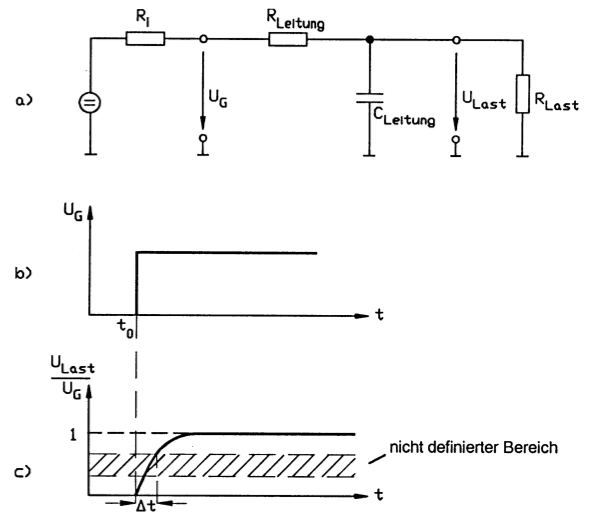
\includegraphics[width=0.6\textwidth]{abbildungen/20160110_impulsbus}
\caption[Impulsverzerrung auf einer Leitung]{Impulsverzerrung auf einer Leitung: a) Ersatzschaltbild der Anordnung b) Ausgangsspannung des Generators c) Empfängerspannung aus \cite[S.~4]{schn06}}
\label{fig:bus_impuls}
\end{figure}

Weitere Bus-Strukturen sind die Baumstruktur, die eine Weiterentwicklung der Linienstruktur ist und auf Abbildung \ref{fig:baum_struktur}. Dabei werden einzelne Linienstrukturen durch Verstärkerelemente, sogenannte  Repeater, miteinander verbunden und es können dadurch größere Flächen als mit der Linienstruktur vernetzt werden. \cite[S.5~f.]{schn06}.
--> Galvanische Trennung und Abschirmung 
Diese Struktur ist insofern interessant, da es also im Rahmen dieser Arbeit Anlage noch eine nachträgliche Erweiterung/Vergrößerung der geplanten Anlage ermöglicht.

Modbus was da oben steht, Teilnehmer kabellängen etc.

\begin{figure}
\centering
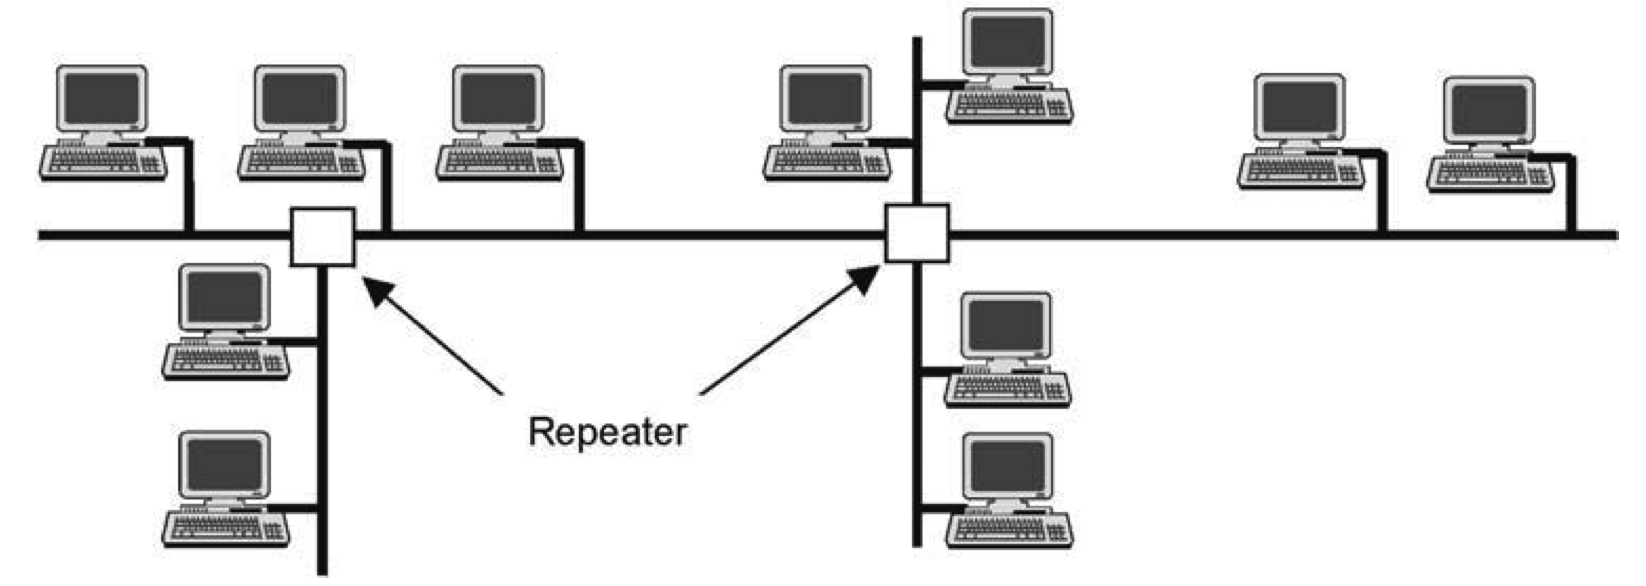
\includegraphics[width=\textwidth]{abbildungen/20160110_baumstruktur}
\caption[Baumstruktur]{Baumstruktur aus \cite[S.~5]{schn06}}
\label{fig:baum_struktur}
\end{figure}

Weitere wichtige Netzwerk Topologien, die für das Verständnis dieser Arbeit keine weitere Relevanz haben, jedoch genannt werden sollten sind die Ring- und die Stern-Struktur. Die Ring-Struktur ist dadurch gekennzeichnet, ein physikalischer Ring mit Zweipunktverbindungen aufgebaut wird in dem über Teilnehmer hinweg kommuniziert wird. Die Stern-Topologie ist durch eine Zentralstation gekennzeichnet, die mit allen Teilnehmer verbunden ist und über die die gesamte Kommunikation abläuft \cite[S.~6f.]{schn06}.

\subsubsection{Elektrisches EIA-485 Netzwerk/Interface}
Hier wird EIA / RS485 dargestellt und abgegrenzt zu RS 232 und RS 422

\subsubsection{Hardware}
Kabel, Belegung

\subsection{Modbus}
Hier wird das Modbusprotokoll nach \cite{mod12} und \cite{mod06ser} und \cite{mod06tcp}  
Und nach hier wird das Modbusprotokoll nach \cite[S.5]{mod12} und \cite[S.5]{mod06ser} und \cite[S.5]{mod06tcp}









\section{Technische Grundlagen zur Modellbildung}
\label{sec:grundlagenmodell}
In diesem Kapitel werden die technischen Grundlagen zur Bildung eines mathematischen Modells des Raumes erläutert.
Themrodym systeme
1. HS thermo
Wärmeübertragung

\subsection{Thermodynamische Systeme}
Im Raummodell müssen Energieströme, genauer betrachtet Wärmeströme, untersucht werden. Um dieses thermodynamischen Vorgänge mit Hilfe von Bilanzierungsgleichungen zu beschreiben, folgt zunächst ein kurze Einführung in die Thermodynamische Systembildung nach \cite[S.~11ff.]{ba12}.

\textit{Thermodynamische Systeme} werden durch den zu untersuchenden Raum abgegrenzt. Sie dienen dem Zweck der Bilanzierung von Massen- und Energieströmen und alles was diesen abgegrenzten Raum an den Systemgrenzen umgibt wird als Umgebung bezeichnet. Die begrenzenden Flächen können gedanklicher, physischer oder beider Natur zugleich sein, wichtig ist jedoch das die Systemgrenzen eindeutig festgelegt sind \cite[S.~11]{ba12}.

Anhand der Eigenschaften von den Systemgrenzen lassen sich die thermodynamischen Systeme weiter differenzieren.
Solche Systeme, deren Grenzen undurchlässig für Materie sind, werden als \textit{geschlossene Systeme} bezeichnet und werden durch eine konstante Stoffmenge innerhalb des Systems gekennzeichnet. Die Grenzen eines geschlossenen Systems sind meistens räumlich anhand eines fixen Volumens definiert, können aber auch beweglich sein, wie z.B. das Volumen einer vorgegebenen Stoffmenge unabhängig von dessen räumlicher Ausdehnung \cite[S.~12]{ba12}.

Sind die Grenzen von thermodynamischen Systemen für Materie durchlässig, werden diese als \textit{offene Systeme} bezeichnet. In der Regel werden diese von Stoffströmen durchflossen und durch räumlich festgelegte Grenzen beschrieben. Diese werden in der Literatur auch als \textit{Kontrollraum} oder \textit{Kontrollvolumen} bezeichnet \cite[S.~12]{ba12}.

Ein \textit{abgeschlossenes System} umfasst in der Regel mehrere Systeme oder ein einzelnes System und dessen Umgebung, so dass es zwischen den Grenzen des abgeschlossenen Systems und seiner Umgebung keine Wechselwirkungen gibt. Die Systemgrenzen werden also so gelegt, dass über sie hinweg keine \acrlong{bzw} keine relevanten\footnote{\textit{Relevant} im Sinne von kaum messbarer Fluss und nicht messbare Auswirkung auf das System.} Flüsse von Materie und Energie \cite[S.~13]{ba12}.

Nach der Abgrenzung folgt die \textit{Beschreibung} von thermodynamischen Systemen und dessen \textit{Eigenschaften}. Diese erfolgt durch \textit{Variablen} und \textit{physikalische Größen} die ein System kennzeichnen. Falls die Variablen feste Werte annehmen werden diese als \textit{Zustandsgrößen} bezeichnet, da sie den \textit{Zustand} eines Systems bestimmen \cite[S.~13]{ba12}. Im Rahmen der Modellbildung in Kapitel \ref{chap:modellbildung} ist es ausreichend die Vorgänge und Effekte auf systemischer Ebene zu betrachten, wodurch sich Modelle mit wenigen Variablen und physikalischen Größen beschreiben lassen.

Die Variablen lassen sich in \textit{äußere Größen}, welche den mechanischen Zustand eines Systems beschreiben\footnote{Zum Beispiel die Koordinaten im Raum oder die relative Geschwindigkeit zum Beobachter)}, und \textit{innere Größen} gliedern, welche den thermodynamischen Zustand, also die Eigenschaften der Materie innerhalb der Systemgrenzen, beschreiben\cite[S.13~f.]{ba12}.

Innerhalb der Grenzen eines thermodynamischen Systems, und damit implizit auch für das Raummodell\footnote{Diese Annahme wird im Kapitel \ref{chap:schlussteil} noch überprüft und kritisch hinterfragt werden müssen} wird \textit{Homogenität} angenommen. Dies bedeutet, dass die physikalischen Eigenschaften, wie \acrlong{zb} Temperatur und Druck, sowie die chemische Zusammensetzung an jeder Stelle innerhalb des Systems homogen ist, also die gleiche Ausprägung besitzt \cite[S.15]{ba12}.

Da wir im Rahmen der Modellbildung Zustände betrachten müssen auch deren Änderungen genauer untersucht werden. Die \textit{Zustandsänderungen} eines Systems werden durch Änderungen von Energie oder Materie über dessen Grenzen hinweg bedingt und finden meist im Austausch der Umgebung statt. Während einer solchen Änderung des Systemzustands wird ein Prozess durchlaufen, der eine zeitliche Abfolge von Ereignissen ist. Eine Änderung des Zustands eines Systems mit der gleichen Wirkung kann also durch verschiedene Prozesse bewirkt werden. Daher beschreibt ein \textit{Prozess} nicht nur die Veränderung des Zustands sondern viel mehr die Beziehungen zwischen einem System und seiner Umgebung \cite[S.21~f.]{ba12}.

Ein Prozess kann aber auch innerhalb eines Systems stattfinden, dass heißt ohne äußere Einwirkungen. Dies geschieht zum durch das Aufheben innerer Hemmungen oder dem Wegfall Zwängen von Außen. Diese Prozesse laufen in abgeschlossenen Systemen meist von selbst ab und streben als Ziel einen ausgeglichenen, also homogenen, Endzustand an. \textit{Ausgleichsprozesse} dienen somit dazu, einen \textit{Gleichgewichtszustand} zu erreichen und repräsentieren Wechselwirkungen zwischen verschiedenen Teilen eines abgeschlossenen Systems. Dabei gleichen sich die Zustandsgrößen von einzelnen Subsystemen wie zum Beispiel der Druck oder die Temperatur einander an. Der Gleichgewichtszustand wird also durch die Zustände in den einzelnen Subsystemen bestimmt und ist dadurch charakterisiert, dass ein System diesen Zustand nicht von sich aus sondern nur durch äußere Eingriffe verlässt, zum Beispiel durch eine Veränderungen in der Umgebung. Die Erfahrung lehrt, dass ein System einem Gleichgewichtszustand entgegen strebt, wenn es sich selbst überlassen wird \cite[S.22~f.]{ba12}.
Im Rahmen der Modellbildung in Kapitel \ref{chap:modellbildung} nehmen diese \textit{Ausgleichsprozesse} eine zentrale Rolle ein, weil der Großteil an Änderungen von einzelnen Zustandsgrößen innerhalb des Raumes darauf zurückgeführt werden können. 

\subsection{Erster Hauptsatz der Thermodynamik}
Der erste Hauptsatz der Thermodynamik wird im Folgenden als allgemeiner Energieerhaltungssatz formuliert und anschließend angewendet um eine Energiebilanzgleichung für geschlossene thermodynamische Systeme zu erhalten.

Der erste Hauptsatz der Thermodynamik erweitert den mechanischen Energieerhaltungssatz um die Energieformen Wärme und innere Energie. Er handelt ganz allgemein vom Prinzip der Energieerhaltung und  dient er der Bilanzierung von Systemen \cite[S.~43]{ba12}.

Die Gesamtenergie eines Systems \gls{e} setzt sich zusammen aus der potenziellen \gls{epot} und kinetischen Energie \gls{ekin} wie in der Mechanik und wird durch die innere Energie \gls{u} ergänzt \cite[S.~49]{ba12}:

\begin{equation}
\label{eq:energie}
E := E_{pot} + E_{kin} + U
\end{equation}

Im weiteren Verlauf der Arbeit werden nur ortsfeste Systeme betrachtet die sich dadurch auszeichnen, dass deren potenzielle Energie  \gls{epot} in etwa konstant ist. Weiterhin erfahren sie im betrachteten Intertialsystem Erde auch nur sehr kleine Änderungen in ihrer Geschwindigkeit, weshalb auch die kinetische Energie \gls{ekin} in etwa konstant ist.  Da die Änderungen der mechanischen Energien in Bezug auf die Änderung der inneren Energie sehr klein sind werden im Folgenden nicht weiter betrachtet und die Gesamtenergie eines Systems \gls{e} vereinfacht und lediglich aus der inneren Energie bestehend angenommen.

Die innere Energie hängt von der spezifischen Wärmekapazität \gls{cp}, der Masse eines Systems \gls{msys} und der Temperatur \gls{t} \acrlong{bzw} \gls{T} ab \cite[S.~54]{ba12}:

\begin{equation}
\label{eq:innereenergie}
U := m*c_p*T=m*c_p*t+u_0,~mit~t=T-T_0
\end{equation}

Nach dem Prinzip der Energieerhaltung, kann die Energie eines Systems also weder erzeugt noch vernichtet werden sondern lediglich durch den Energietransport über dessen Grenzen hinweg verändert werden. Daraus ergeben sich folgende qualitative Formen des Energietransports \cite[S.~48f.]{ba12}:

\begin{itemize}
	\item Die Arbeit \gls{w}, die entweder von oder an einem System verrichtet wird, in differentieller Form die Leistung \gls{p}.
	\item Die Wärme \gls{q}, die entweder in das System hinein- oder herausfließt, in differentieller Form der Wärmestrom \gls{qdot}.
	\item Der Transport von Materie, also das Einbringen oder Wegnehmen von Masse \gls{m} eines System, in differentieller Form die Materialflüsse \gls{mdot}.
\end{itemize}

Mit der zuvor getroffenen Annahme, dass die innere Energie der des Systems entspricht, und unter Beachtung der Vorzeichenkonvention, welche besagt dass zugeführte Energie positiv und abgeführte Energie negativ zu bewerten ist, lassen sich die Änderungen der Energie eines Systems mit der folgenden Gleichung quantitativ beschreiben \cite[S.~54]{ba12}:

\begin{equation}
\label{eq:hauptsatz}
\begin{split}
\Delta U & = Q + W + m_{in}*c_{p}*T_{in}-m_{out}*c_{p}*T_{out} \\ ~& \mathrm{beziehungsweise~in~differentieller~Form}\\
\frac{dU}{dt}=\dot{U} & =\dot{Q}+P+\sum\dot{m}_{in}*c_{p}*T_{in}-\sum\dot{m}_{out}*c_{p}*T_{out}
\end{split}
\end{equation}


%Noch einmal überarbeiten

\subsection{Wärmeübertragung}

Wärmeströme spielen bei der Modellbildung in Kapitel \ref{chap:modellbildung} eine wichtige Rolle, daher ist eine genauere Betrachtung dieser unumgänglich und im Folgenden werden die Grundlagen dazu erläutert.

Die Definition von Wärmeübertragung ist nach \cite[S.~1]{bo14} \Gun [...] der Transfer der Energieform Wärme aufgrund einer Temperaturdifferenz. \Gun Die Definition umfasst also einen zuvor beschriebenen Ausgleichsprozess und eine Änderung der inneren Energie eines thermodynamischen Systems.
Die Wärmeübertragung kann nach \textit{Nußelt}\footnote{Beschrieben in seinem Aufsatz \Gun Das Grundgesetz des Wärmeüberganges\Gob , 1915.} grundsätzlich durch zwei verschiedene Arten stattfinden \cite[S.~3f.]{bo14}:

\begin{itemize}
	\item Durch Strahlung, bei der die Übertragung von Wärme ohne stofflichen Träger durch elektromagnetische Wellen zwischen Oberflächen erfolgt. Weil diese Art der Wärmeübertragung keine Relevanz für die weiteren Betrachtungen hat wird an dieser Stelle nicht weiter darauf eingegangen. 
	\item  Durch Wärmeleitung, die sich wiederum in die Wärmeübertragung zwischen ruhenden Stoffen, und die Konvektion, die eine Wärmeübertragung zwischen einem ruhenden und einem strömenden Fluid beschreibt, aufteilen lässt. 
\end{itemize}

Die übertragene Wärmemenge ist bei der reinen Wärmeleitung lediglich von den Stoffeigenschaften und der Temperaturdifferenz abhängig, bei der Konvektion hingegen, unabhängig davon ob erzwungen oder frei, hängt sie von der Strömung der Fluide ab. Die Konvektion ist ein Effekt zusätzlich zur reinen Wärmeleitung auftritt und ist im weiteren Verlauf der Arbeit nicht relevant und wird deshalb nicht detaillierter ausgeführt \cite[S.~3f.]{bo14}.
Erfolgt der Wärmetransport stationär, dass heißt er ist von äußeren Anregungen bedingt und unabhängig von der Zeit, lässt er sich qualitativ einfach als konstanter Wärmestrom \gls{qdot} beschreiben und gibt an wie viel Wärme pro Sekunde übertragen wird \cite[S.~5ff.]{bo14}. Der Wärmestrom ist wie zuvor bereits erwähnt von den Stoffeigenschaften abhängig, welche von der Wärmedurchgangszahl \gls{uwert}\footnote{Der U-Wert wurde bis zu der Umstellung auf die europäischen Prüfnormen 2003 als k-Wert bezeichnet und ist unter dieser Bezeichnung noch häufig in der Literatur zu finden \cite[S.1~f.]{sa04}} und der Austauschoberfläche \gls{A}, an der der Wärmeaustausch stattfindet. Typische U-Werte für verschiedene Materialien und Komponenten finden in der einschlägigen Literatur und beziehen sich bei der Übertragung durch eine Wand im europäischen Raum auf die Außenfläche \cite[S.~28]{bo14}. Damit lässt sich der Wärmestrom unter Berücksichtigung der Abhängigkeiten durch die kinetische Kopplungsgleichung quantifizieren \cite[S.~6f.]{bo14}:

\begin{equation}
\label{eq:qdot}
\dot{Q} := u*A*(t_{1}-t_{2})
\end{equation}

Unterschiedliche geometrische Ausprägungen, wie zum Beispiel ein Wärmeaustausch durch eine Wand oder ein Rohr hindurch, finden damit implizit bei der Austauschoberfläche Berücksichtigung.

% Here we go after OSI

\section{Technische Grundlagen zur Solartechnik}
\subsection{Klima}\subsection{Sonnenbahn}
\subsection{Sonnenstrahlung}


